%Centralizar verticalmente.
\newenvironment{midpage}{\vspace*{\fill}}{\vspace*{\fill}}
%Centralizar horizontalmente.
\newenvironment{midline}{\hspace*{\fill}}{\hspace*{\fill}}
\documentclass[12pts]{article}
\usepackage[utf8]{inputenc}
%Pacote para colocar cor no código.
\usepackage{color}
\definecolor{light-gray}{gray}{0.95}
%Pacote para inserir código.
\usepackage{listings}
\lstset{
    numbers=left,
    tabsize=2,
    backgroundcolor=\color{light-gray},
}\title{
	Prática de Eletrônica Digital 1 - (119466)
	\singlespacing
		Turma E (Unb - Gama)
	\singlespacing
	\begin{midpage}
	\begin {large}
		Relatório Experimento 4
		\singlespace
		Circuitos Codificadores
	\end {large}
	\end{midpage}
}
\date{Setembro 23, 2016}
\usepackage{indentfirst}
\usepackage{setspace}
\usepackage{verbatim}
\usepackage[pdftex]{hyperref}
\usepackage{graphicx}
\begin{document}
\maketitle	
%\vspace{100 mm}
\begin{center}

\begin{tabular}{|c|l|r|}
\hline
Nome & Matrícula & Assinatura\\
\hline

Arthur Temporim & 14/0016759 & \\
\hline	
Eduardo Nunes & 14/0056189 & \\

\hline	
\end{tabular}

\end{center}


\newpage

\section{Sumário}

\begin{itemize}
	\item Introdução
	\singlespacing
	\item Experimentos
	\singlespacing
	\item Discussão
	\singlespacing
	\item Conclusões 
	\singlespacing
	\item Referências Bibliograficas
	\singlespacing
	%\item Diagramas esquemáticos
\end{itemize}

\newpage


\section{Introdução}
\iffalse
Introdução, indicando a delimitação do tema, apresentando a justificativa descrevendo o propósito do relatório.
\fi

	 Neste relatorio e apresentado o resultado do experimento realizado na aula da prática da eletrônica digital 1. São apresentados os mapas de Karnaugh, o código vhdl e a saída em forma de onda. Para este experimento foi utilizado a ferramenta \textit{Ise design suite}.

\section{Experimentos}
\iffalse
Parte Experimental, descrevendo os passos realizados, dificuldades e soluções para os problemas encontrados. Aqui, deve-se apresentar uma descrição dos resultados encontrados em forma de figuras, gráficos e tabelas.
\fi

\subsection{Experimento 01}
\singlespacing

	O primeiro experimento tratou-se da implementação de um circuito a partir da tabela verdade. A dupla teve de identificar os mintermos e elaborar mapas de Karnaugh para alcançar as funções lógicas simplificadas.
	
	Para a realização do experimento em sala de aula, foi despresado os valores hexadecimais referenstes ao display de 7 segmentos, ou seja, que utilizassemos apenas os dez primeiros valores da tabela que representam os algarismos de 0 à 9. 
	
	Segue abaixo, respectivamente: Mapas de Karnaugh, Código vhdl, diagrama esquemático e saída obtida em forma de onda.
\singlespacing

\subsection{Mapas de Karnaugh}

\begin{table}[h]
\begin{center}
	\begin{tabular}{|l|l|l|l|l|}
		\hline
		\textbf{AB/CD} & \textbf{00} & \textbf{01} & \textbf{11} & \textbf{10}\\
		\hline
		\textbf{00} & 1 & 0 & 1 & 1\\
		\hline
		\textbf{01} & 0 & 1 & 1 & 1\\
		\hline
		\textbf{11} & X & X & X & X\\
		\hline
		\textbf{10} & 1 & 1 & X & X\\
		\hline
	\end{tabular}
\end{center}
	\caption{Mapa de Karnaugh da saida A. Equação: A = C + A + !B!D + BD }
	\end{table}
	\singlespacing

\begin{table}[h]
\begin{center}
	\begin{tabular}{|l|l|l|l|l|}
		\hline
		\textbf{AB/CD} & \textbf{00} & \textbf{01} & \textbf{11} & \textbf{10}\\
		\hline
		\textbf{00} & 1 & 1 & 1 & 1\\
		\hline
		\textbf{01} & 1 & 0 & 1 & 0\\
		\hline
		\textbf{11} & X & X & X & X\\
		\hline
		\textbf{10} & 1 & 1 & X & X\\
		\hline
	\end{tabular}
\end{center}
	\caption{Mapa de Karnaugh da saida B. Equação: B = !B + !C!D + CD }
\end{table}
	
\singlespacing

\begin{table}[h]
\begin{center}
	\begin{tabular}{|l|l|l|l|l|}
		\hline
		\textbf{AB/CD} & \textbf{00} & \textbf{01} & \textbf{11} & \textbf{10}\\
		\hline
		\textbf{00} & 1 & 1 & 1 & 0\\
		\hline
		\textbf{01} & 1 & 1 & 1 & 1\\
		\hline
		\textbf{11} & X & X & X & X\\
		\hline
		\textbf{10} & 1 & 1 & X & X\\
		\hline
	\end{tabular}
\end{center}
	\caption{Mapa de Karnaugh da saida C. Equação: C = !C + B + D }
	\end{table}
	\singlespacing
	
\begin{table}[h]
\begin{center}
	\begin{tabular}{|l|l|l|l|l|}
		\hline
		\textbf{AB/CD} & \textbf{00} & \textbf{01} & \textbf{11} & \textbf{10}\\
		\hline
		\textbf{00} & 1 & 0 & 1 & 1\\
		\hline
		\textbf{01} & 0 & 1 & 0 & 1\\
		\hline
		\textbf{11} & X & X & X & X\\
		\hline
		\textbf{10} & 1 & 1 & X & X\\
		\hline
	\end{tabular}
\end{center}
	\caption{Mapa de Karnaugh da saida D. Equação: D = A +B!CD + C!A!B + !B + !D }
	\end{table}
	\singlespacing
	
\begin{table}[h]
\begin{center}
	\begin{tabular}{|l|l|l|l|l|}
		\hline
		\textbf{AB/CD} & \textbf{00} & \textbf{01} & \textbf{11} & \textbf{10}\\
		\hline
		\textbf{00} & 1 & 0 & 0 & 1\\
		\hline
		\textbf{01} & 0 & 0 & 0 & 1\\
		\hline
		\textbf{11} & X & X & X & X\\
		\hline
		\textbf{10} & 1 & 0 & X & X\\
		\hline
	\end{tabular}
\end{center}
	\caption{Mapa de Karnaugh da saida E. Equação: E = !D!B + C!D }
	\end{table}
	\singlespacing

\begin{table}[h]
\begin{center}
	\begin{tabular}{|l|l|l|l|l|}
		\hline
		\textbf{AB/CD} & \textbf{00} & \textbf{01} & \textbf{11} & \textbf{10}\\
		\hline
		\textbf{00} & 1 & 0 & 0 &0\\
		\hline
		\textbf{01} & 1 & 1 & 0 & 1\\
		\hline
		\textbf{11} & X & X & X & X\\
		\hline
		\textbf{10} & 1 & 1 & X & X\\
		\hline
	\end{tabular}
\end{center}
	\caption{Mapa de Karnaugh da saida F. Equação: F = A + B!C + !C!D + B!D }
	\end{table}
	\singlespacing
	
\begin{table}[h]
\begin{center}
	\begin{tabular}{|l|l|l|l|l|}
		\hline
		\textbf{AB/CD} & \textbf{00} & \textbf{01} & \textbf{11} & \textbf{10}\\
		\hline
		\textbf{00} & 0 & 0 & 1 & 1\\
		\hline
		\textbf{01} & 0 & 0 & 0 & 1\\
		\hline
		\textbf{11} & X & X & X & X\\
		\hline
		\textbf{10} & 1 & 1 & X & X\\
		\hline
	\end{tabular}
\end{center}
	\caption{Mapa de Karnaugh da saida G. Equação: G = A + C(B + !D) }
	\end{table}
	\singlespacing

\clearpage
\subsection{Código VHDL}
\lstinputlisting[language=vhdl]{projetos/projeto1/projeto1.vhd}

\clearpage
\subsection{Diagrama Esquemático}
\begin{figure}[!htb]
  \centering
  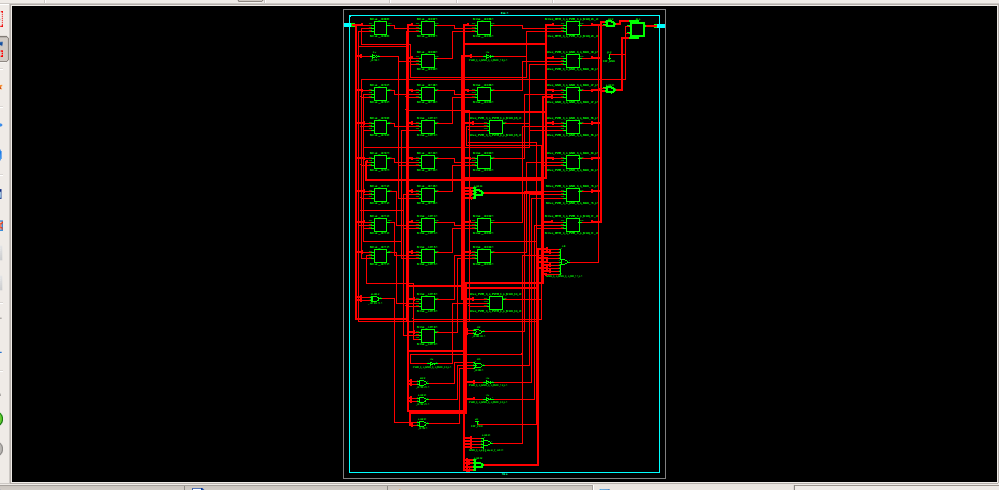
\includegraphics[scale=0.6]{imagens/circuito}
  \caption{Diagrama do circuito codificador - Ise Design Suite 14.7}	
  \label{figRotulo}
\end{figure}

\newpage
\subsection{Diagrama de Onda}

\begin{figure}[!htb]
  \centering
  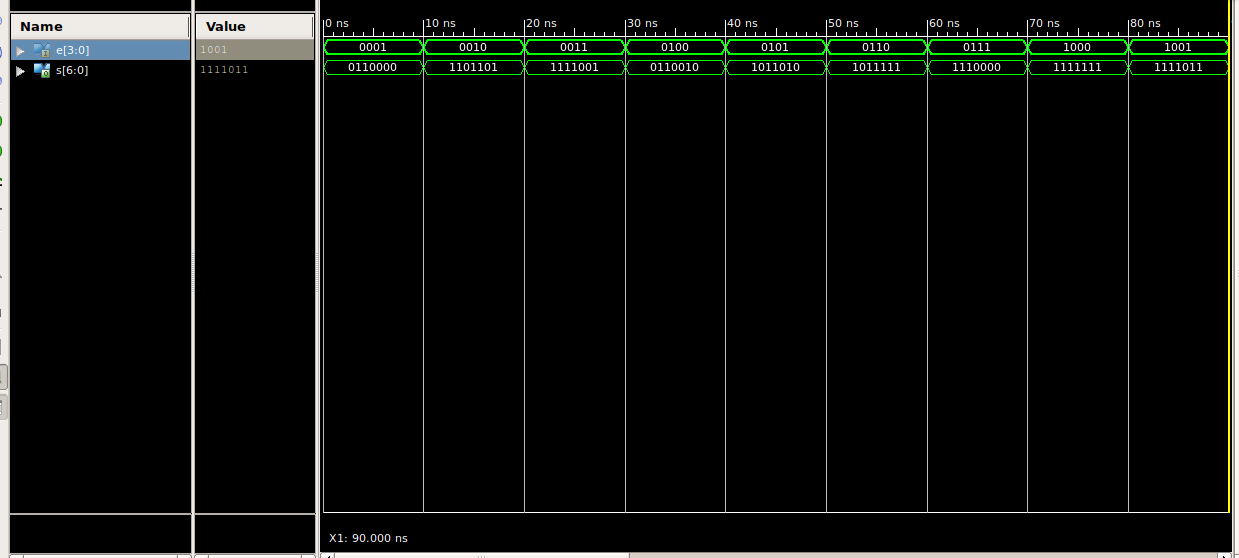
\includegraphics[scale=0.35]{imagens/onda}
  \caption{Diagrama de ondas do circuito codificador - Ise Design Suite 14.7}
  \label{figRotulo}
\end{figure}
\newpage

\section{Discussão}
\iffalse
Discussão sobre os resultados encontrados, comentando detalhadamente as medições realizadas e dando a devida interpretação destas, informando se os objetivos da experimento foram alcançados. Esta é uma das partes mais importantes do relatório: aqui, há oportunidade para expressar os conhecimentos adquiridos na prática e fazer a interrelação com os fundamentos teóricos.
\fi

	Com a realização deste experimento foi possível adquirir conhecimento a respeito do mapa de Karnaugh. Também foi possível entender que a \textit{concepção} de um circuito de forma manual e implementação em código VHDL pode ser bem distinta, porém o objetivo alcançado é o mesmo. Na realização do experimento foram simplificadas todas as funções lógicas, porém a implementação no vhdl foi feita com estruturas condicionais.

	Todas os resultados apresentados nas saídas do experimento foram de acordo com o esperado.

\section{Conclusões}
\iffalse
Conclusões, mostrando os êxitos e eventuais problemas encontrados na realização do experimento, indicando as limitações, apresentando recomendações e/ou sugestões.
\fi

	Neste quarto relatório foi possível realizar o experimento com êxito. A compreensão da necessidade de simplificação de funções lógicas pode ser alcançada juntamente com o aprendizado de novas formas de implementação de circuitos em VHDL.



\section{Referências Bibliográficas}
\iffalse
Referencias Bibliográficas, relacionadas e citadas de acordo com as normas da ABNT.
\fi
Prática de Eletrônica Digital I 2016.2 professores Henrique Marra Taira Menegaz,Leonardo Aguayo, Lourdes Mattos Brasil, Marcus Vinícius Chaffim Costa, Mariana Costa Bernardes Matias. UnB - FGA Agosto de 2015.

\iffalse
\section{Diagramas Esquemáticos}
Diagramas Esquemáticos. Todos os diagramas devem ser inseridos ao final do relatório em páginas separadas do texto, indicando a identificação do circuito, autor, revisor, versão e datas relevantes.
\fi
\newpage

\end{document}

%Exemplo de imagem
\iffalse
\begin{figure}[!htb]
  \centering
  \includegraphics[scale=0.3	]{nome_da_imagem}
  \caption{Descrição}
  \label{figRotulo}
\end{figure}
\fi

% Exemplo de tabela.
\iffalse
\begin{tabular}{|c|r|}
\hline
Material Utilizado & Quantidade\\
\hline
Cabo Banana-Banana & 2  \\
\hline
Fios de cobre & x \\
\hline
Cabo coaxial & 3  \\
\hline
CI 74HC00   & 1 \\
\hline
CI 74LS00   & 1 \\
\hline
Protoboard & 2 \\
\hline
Fonte de tensão MPL-3305M & 1 \\
\hline	
Multímetro Digital  & 1 \\
\hline
Gerador de funçoes iCEL modelo GV-2002 & 1 \\
\hline
Osciloscopio BK 2530 & 1 \\
\hline
\end{tabular}
\singlespacing
\fi

